\documentclass[11pt]{article}   % Mandatory
\usepackage[T1]{fontenc}        % Support for fonts with æøå and other foreign characters.
\usepackage[utf8]{inputenc}     % Support for UTF-8 encoded input documents
\usepackage{fullpage}
\usepackage{graphicx}           % Support for including graphics as png, gif, and jpeg
\usepackage{amssymb}            % Support for alterantive symbols
\usepackage{amsmath}            % Support for mathematical symbols
\usepackage{listliketab}        % Support for tabulated lists
\usepackage{enumitem}           % Support for indented description items and more
\usepackage[parfill]{parskip}   % Support for American style paragraphs
\usepackage{color}              % Support for colored text
\usepackage{listings}           % Support for code listings
\usepackage{nameref}            % Enables refernces to names.
\usepackage{makeidx}            % For creating indexes
\usepackage{wasysym}            % For symbols as \smiley
\usepackage{hyperref}        	% For using URLs
\usepackage{utility/petri}      % For doing petrinet vector graphics
\usepackage{xspace}             % For adding a space only when necessary. See ePNS command below.
\newcommand{\epns}{\textbf{Extended Petri net Simulator}\xspace}
\newcommand\writer[1]{\nobreak\begin{flushright}\small\textbf{Author: \large\textit{#1}}\end{flushright}}
\makeindex

\def\signed #1{{\leavevmode\unskip\nobreak\hfil\penalty50\hskip2em
  \hbox{}\nobreak\hfil(#1)%
  \parfillskip=0pt \finalhyphendemerits=0 \endgraf}}

\newsavebox\mybox
\newenvironment{aquote}[1]
  {\savebox\mybox{#1}\begin{quotation}}
  {\signed{\usebox\mybox}\end{quotation}}

\title{System Specification\\ \epns}
\author{Group A}
\date{\today}

\begin{document}o
\maketitle

\begin{abstract}
This document includes the requirements for the Software Engineering 2 project, which consists of an Extended Petri net software system.
\end{abstract}

\tableofcontents \newpage

\section{Introduction}
\writer{Thibaud, Albert}

\begin{quotation}
Petri nets, as graphical and mathematical tools, provide a uniform environment for modelling, formal analysis, and design of discrete event systems. \footnote{Petri Nets and Industrial Applications: A Tutorial. Richard Zurawski, MengChu Zhou.}
\end{quotation}

Petri nets are used as a means to model systems, but, as they are a mathematical concept, they are not always easy to understand for the ordinary user. Complex systems can be modelled with Petri nets, and usually, this would be an engineer's job. Even though engineers can easily create and understand their own Petri nets, every team member in a company would like to be able to understand what a Petri net is about without having any knowledge of the concepts behind them.

Therefore, the project aims at creating a 3D visualisation from a Petri net, to allow non-Petri net experts to actually to understand how the model works and validate a system.

However, Petri nets were not intended to have a 3D representation. For instance, there is no graphical concept or way to say that a particular Petri net would look like a train track because it was used to model a railway system. 

Thus, our goal for this project is the following: Providing an extension to Petri net models to make their 3D visualisation possible. For this purpose, we have imagined a simple link between a Petri net and a 3D visualisation.

\subsection{Conventions}

The priority of the requirements in Section \ref{sec:system-features} and \ref{sec:non-functional} will be indicated by the keywords \textbf{shall}, \textbf{should} and \textbf{would be nice}:

\begin{itemize}
	\item \textbf{Shall}: Requirements that must be implemented as a minimum, resources must be allocated to these requirements.
	\item \textbf{Should}: Requirements that add more functionality to the software, but are not the core required to work, if possible, resources will be allocated.
	\item \textbf{Would be nice}: Requirements considered good ideas and would be implemented if there are sufficient resources or in later versions of the software.
\end{itemize}

\subsection{Audience}

The audience of this document are persons affiliated with the company that models and simulates Petri net, developers of the system and final users of the Extended Petri net Simulator.
\newpage
\section{Overall description}
%\writer{Thibaud}

This section describes the software and provides a brief explanation on how the system works.

\subsection{What are Petri nets?}

Petri nets are a graphical and mathematical modelling tool for describing concurrent and distributed systems. Some examples of their applications are workflow management, embedded systems or traffic control. The main advantages of Petri nets are their graphical notation, their simplicity on the semantics, and their rich theory for analysing their behaviour. However, using the Petri net graphical notation for understanding a complex system is quite hard, and thus a user-oriented visualization is required in a way that is understandable to users which are not necessarily familiar with Petri nets.


\begin{figure}[htp]
\begin{center}
  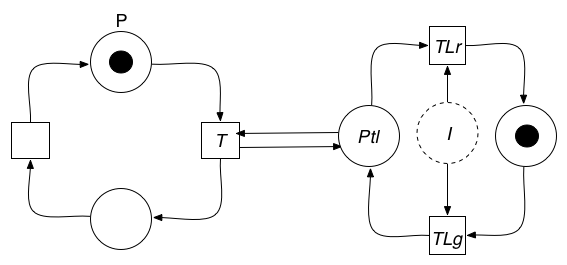
\includegraphics[width=0.8\textwidth]{image/petrinet_diagram.png}
  \caption{An example of a basic Petri net}
  \label{fig:petrinet}
\end{center}
\end{figure}

Figure \ref{fig:petrinet} presents an example of a basic Petri net. There are four different elements:

\begin{itemize}
\item Places: graphically represented by circles, represent conditions.
\item Transitions: graphically represented by squares, represent events.
\item Arcs: indicate which places are preconditions/postconditions for which transitions.
\item Tokens: graphically represented by the dots, represent the elements that move in the Petri net along the places through the transitions.
\end{itemize}


Furthermore, we can see the example of Figure \ref{fig:petrinet} as a model for a railway with a traffic light. The token in Place P1 represents a train moving on a railway. When this train arrives to Place P1, the transition T will fire if the conditions are met. The only condition for a transition to be fired is that a token should be present on each of the incoming places of the transition.

In this scenario, the conditions are not met, as the required token in Place Ptl is missing. The visualization of this scenario would be a traffic light with a red light. If Place I had a token on it, it would generate a token that will turn the traffic light to green and thus the train will move. 

%If a user clicks on the Place I, it would generate a token that will turn the traffic light to green and thus the train will move.

With the aim of creating a visualization of the scenarios for the above Petri net model, an application tool is needed in order to allow the user to define where each of the elements are represented in the 3D world (geometry editor) as well as how these elements are represented (shape) and how they behave (animation). 

\subsection{Adding geometry to Petri nets}
The problem this project is tackled with is simple: We need a way to link the Petri net model to a 3D visualisation, this is, to add extra information so that it can be visualized. Once a Petri net model is created and its real life design is well-designed in the user's mind, what we call a "Geometry" and "Appearance" are created.

For this purpose, there is a need of a geometry editor which will be used to assign a two dimensional location to the elements defined in the Petri net, and of an appearance editor to take care of the shape of the elements.

\subsection{Adding appearance to Petri net objects}
\label{sec:appearance}

Once the geometry problem is solved, a shape for each object should be defined. For instance, if places represent tracks, the shape, texture and other attributes should be linked to that object.

For this purpose, there is a need of an appearance editor which will be used to assign 3D visualization features to the elements defined in the Petri net.

\subsection{Configuration}

Before running the simulation, a definition of how the previous models are connected is needed. This is done in the configuration step as well as the validity check for the Petri net's connections to the geometry. 

\subsection{Simulating Petri nets}
The next step in visualizing Petri nets is add descriptive visuals. With the information provided by the Petri net, geometry and appearance as defined in the configuration file, the simulation is set up.

\begin{figure}[htp]
\begin{center}
  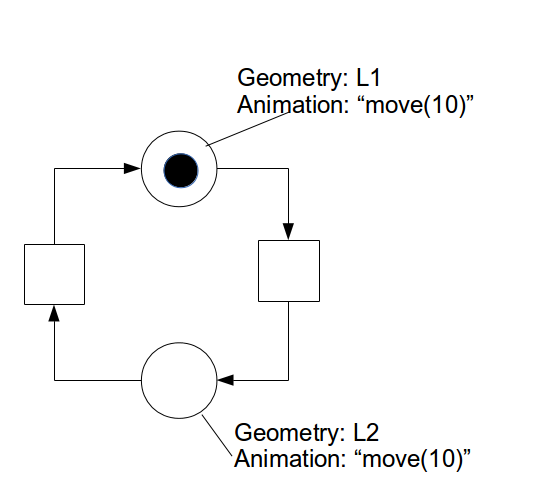
\includegraphics[width=0.4\textwidth]{image/example_petrinet.png}
  \caption{A simple extended Petri net}
  \label{fig:example_petrinet}
\end{center}
\end{figure}

\begin{figure}[htp]
\begin{center}
  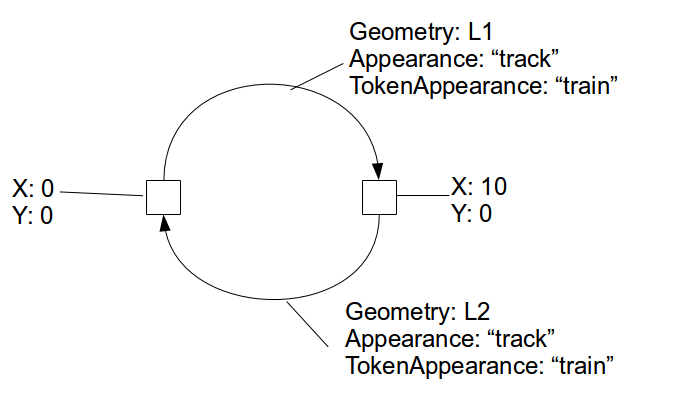
\includegraphics[width=0.4\textwidth]{image/example_petrinet_geometry.png}
  \caption{A simple geometry}
  \label{fig:example_petrinet_geometry}
\end{center}
\end{figure}

Using 3D models, textures and animations, the Petri net becomes easier to understand for the user. Continuing with the railway example, tokens become trains that move on tracks, which are places. As the tokens move from place to place, the train is animated in the 3D visualization along the tracks.

Figure \ref{fig:3steps}  shows how a simple 3D simulation of a train track and a train is made out of Petri net model and a simple geometry. Place P1 references L1 as its geometry and also has the shape of a track. The token on place P1 has the shape of a train and it moves with an animation defined by the place P1.

\subsection{General product description}

The overall description is a brief introduction to how our software is designed. For this purpose, it contains a description of the actors involved in its use, and also a description of how the software works. \newline

The following persons are all actors of our software:

\begin{itemize}
  \item Petri net engineer: An engineer whose role is to design and develop a Petri net which suits the company needs. \newline
  For instance, this could be an engineer working at a railway company and in charge of modelling the railway system using Petri nets.
  \item End user: An actor to whom the Petri net 3D-Visualization would be presented, or an actor who is in charge of presenting the Petri net to another. \newline
	For instance, this could be a manager wanting to see what a Petri net represents. 
\end{itemize}

The software is built around three different concepts: 

\begin{itemize}
  \item Editors: A component responsible for handling the creation and design of one of our models. \newline
	For example: A Petri net editor to create a Petri net model. \newline
	An editor is presented to the user as a GUI in an Eclipse window.
  \item Simulator: A simulator is, as its name says, a component capable of simulating a Petri net.
	The simulator is handling all the decisions regarding the Petri net and its behaviour. 
	It then communicates the decisions to a 3D Engine responsible for the visualization.
  \item 3D Engine: A 3D Engine is responsible for the visualization of a Petri net in three dimensions.
	It receives input from the Petri net simulator, and also communicates to the simulator when a user performs a certain type of action. \newline
	For example: the user clicks on a specific Place of the Petri net, this triggers a message from the 3D Engine to the Petri net simulator 
\end{itemize}
\newpage
Figure \ref{fig:system_diagram}. shows the different components of our system and their connections.

\begin{figure}[htp]
\begin{center}
  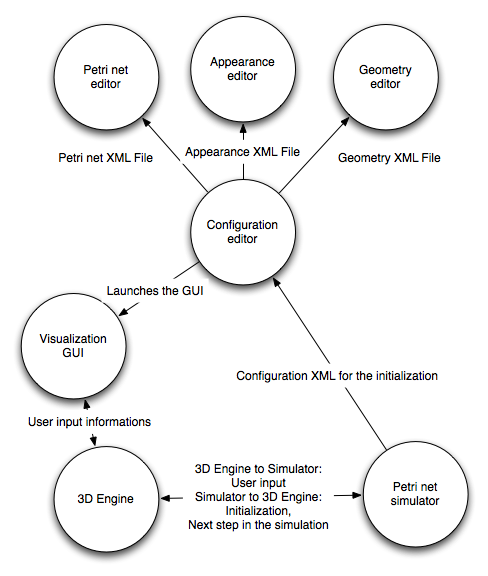
\includegraphics[width=0.6\textwidth]{image/system_design.png}
  \caption{System design}
  \label{fig:system_diagram}
\end{center}
\end{figure}

\subsection{Basic functionality}


This software allows the engineers to create a Petri net 3D Visualization using a combination of the different editors built for this project.
The files created with each of the following editors are to be combined using the configuration editor: \newline
Petri net editor, Geometry editor, Appearance editor. 

Once the files are linked together in the configuration editor, a 3D Visualization can be launched in the workbench. \newline

The simulator then initializes the 3D Engine with all the informations needed for the visualization. The 3D Engine then relies on the simulator to know which next move it should perform on the Petri net. \newline
To interact with the simulation, the user can either click or press certain keyboard buttons in the GUI for the visualization. \newline



\section{System Features}
\label{sec:system-features}

In this section, the main features of the components will be discussed, as well as possible features that could be implemented in future releases of the product.
The main functionality needed by each component in order for the project to work will be explained into more detail. \newline
The main use cases of the system components are also provided in each subsection in order to describe how the system will be used by the final user. 

\subsection{Conventions}

The priority of the requirements in Section \ref{sec:system-features} and \ref{sec:non-functional} will be indicated by the keywords \textbf{shall}, \textbf{should} and \textbf{would be nice}:

\begin{itemize}
	\item \textbf{Shall}: Requirements that must be implemented as a minimum; resources must be allocated to these requirements.
	\item \textbf{Should}: Requirements that add more functionality to the software, but are not the core required to work; if possible, resources will be allocated.
	\item \textbf{Would be nice}: Requirements considered good ideas and would be implemented if there are sufficient resources or in later versions of the software.
\end{itemize}


\subsection{Petri net editor}
\label{sec:sf-petrinet}
\writer{Albert}

The Petri net editor is a component that will extend the features provided by the \textit{ePNK}, in order to fulfil the requirements of the project. The extended features include \textit{Input Places} and the definition of links between geometry and animation components.

\subsubsection{Functional Requirements}

\begin{enumerate}
	\item The Petri net editor \textbf{shall} allow the user to create, edit and delete Places.
	\item The Petri net editor \textbf{shall} allow the user to create, edit and delete Tokens inside Places.
	\item The Petri net editor \textbf{shall} allow the user to create, edit and delete Transitions.
	\item The Petri net editor \textbf{shall} allow the user to create, edit and delete Arcs. An arc \textbf{shall} connect a Place to a Transition or vice versa.
	\item The Petri net editor \textbf{shall} allow the user to define a Geometry label to a Place.
	\item The Petri net editor \textbf{shall} allow the user to define an Appearance label to a Place.
	\item The Petri net editor \textbf{shall} allow the user to define an Input Place label to a Place.
	\item The Petri net editor \textbf{shall} allow the user to define an Animation label to a Place.
	\item The Petri net editor \textbf{shall} allow the user to save and load a Petri net model.
	\item The Petri net editor \textbf{shall} create a Petri net file in a format that can be read by the Simulator.
	\item It \textbf{would be nice} that the Petri net editor allowed the user to undo and redo actions.
	\item It \textbf{would be nice} that the Petri net editor allowed the user to copy and paste.
\end{enumerate}

\subsubsection{Use cases}

The features are shown in Figure~\ref{fig:use-cases-petri-net-editor}.

\begin{figure}[htp]
\begin{center}
  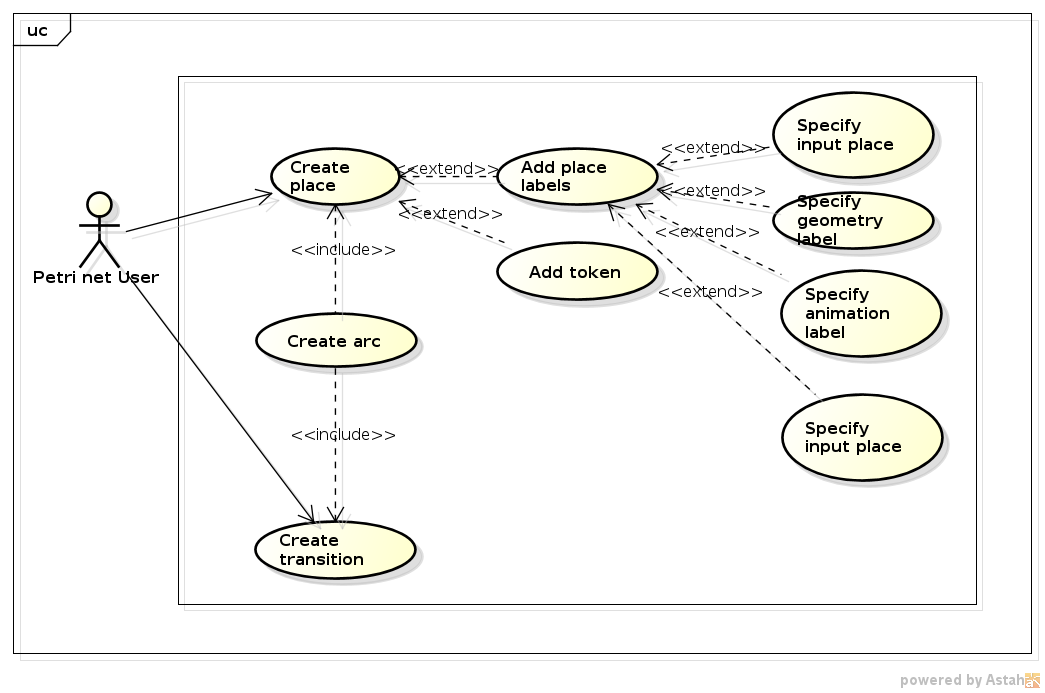
\includegraphics[width=0.8\textwidth]{image/uc-petri-net.png}
  \caption{Use cases for the Petri net Editor}
  \label{fig:use-cases-petri-net-editor}
\end{center}
\end{figure}
\subsection{Geometry editor}
\label{sec:sf-geometry}

Geometry editor is a tool to create and edit geometry. Geometry consists of geometry objects. They are either lines or points. Geometry editor has following requirements.

\subsubsection{Functional Requirements}

\begin{enumerate}
	\item Geometry editor \textbf{shall} allow user to create, edit and delete points.
	\item Geometry editor \textbf{shall} allow user to create, edit and delete define point as inputPoint, Connector or bendPoint.
	\item Geometry editor \textbf{shall} allow user to create, edit and delete lines by using connectors and bendPoints.
	\item Geometry editor \textbf{shall} allow user to load and save geometry file.
	\item Geometry editor \textbf{shall} allow user to define labels for geometry objects.
	\item Geometry editor \textbf{shall} create unique IDs for geometry objects.
	\item Geometry editor \textbf{should} allow user to create parametric curved lines.
	\item Geometry editor \textbf{should} allow user to use undo and redo.
	\item Geometry editor \textbf{should} allow user to use copy, paste and cut geometry objects.
	\item Geometry editor \textbf{should} have a Graphical User Interface.
	\begin{enumerate}
		\item Geometry editor \textbf{should} have drag and drop interface.
		\item Geometry editor \textbf{should} enable editing of geometries with a text input.
		\item It \textbf{would be nice} if the geometry editor allows user to create different kinds of parametric curved lines, such as Catmull-rom spline and Bézier-curves.
		\item It \textbf{would be nice} if the geometry editor allows user to zoom and pan the geometry canvas.
		\item It \textbf{would be nice} if the geometry editor allows user select multiple geometry objects simultaneously.
		\item It \textbf{would be nice} if the geometry editor allows user to load multiple geometries on same canvas.
		\item It \textbf{would be nice} if the geometry editor allows user select multiple geometry objects simultaneously.
		\item It \textbf{would be nice} if the geometry editor allows user to rotate and scale geometry objects.
		\item It \textbf{would be nice} if the geometry editor allows user to toggle visibility of geometry objects while using geometry editor.
	\end{enumerate}
	\item It \textbf{would be nice} if you could specify a Petri ned model from which the geometry is being specified from and it is validated.
\end{enumerate}

\subsubsection{Use cases}

The uses of geometry editor is summed up in the use case diagram in Figure~\ref{fig:use-cases-geometry-editor}.

\begin{figure}[htp]
\begin{center}
  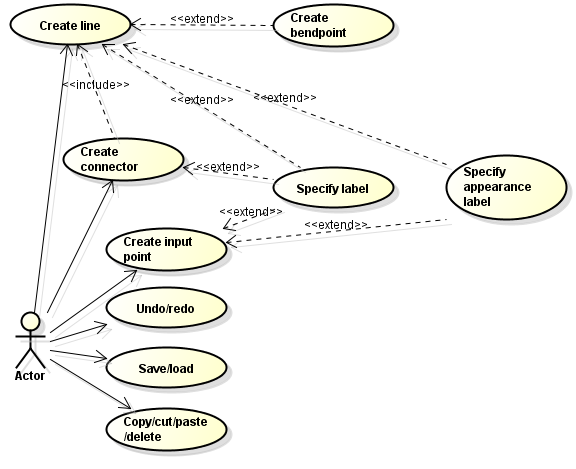
\includegraphics[width=0.5\textwidth]{image/uc-geometry.png}
  \caption{Use cases for the Geometry editor}
  \label{fig:use-cases-geometry-editor}
\end{center}
\end{figure}
\subsection{Appearance Editor}
\label{sec:sf-appearance}

The Appearance Editor is a component that will allow the user to add visual information such as shapes and textures to the Petri net elements to be simulated. The connection between the appearance files and the Petri net elements will be done via the \textit{appearance label}. 

\subsubsection{Functional Requirements}

\begin{enumerate}
\item The Appearance Editor \textbf{shall} allow the user to link appearance labels to 3D objects by choosing a predefined file.
\item The Appearance Editor \textbf{shall} allow the user to link appearance labels to textures by choosing a predefined file.
\item The Appearance Editor \textbf{shall} create an Appearance file in a format that can be read by the Configuration Editor.
\item The Appearance Editor \textbf{shall} allow the user to load an Appearance file.
\item The Appearance Editor \textbf{shall} allow the user to save an Appearance ]file.
\item \textbf{It would be nice} to allow the user to load a Petri net file in order to retrieve all the appearance labels.     
\end{enumerate}

\subsubsection{Use cases}

The features described above are shown in Figure~\ref{fig:use-cases-appearance-editor}.

\begin{figure}[htp]
\begin{center}
  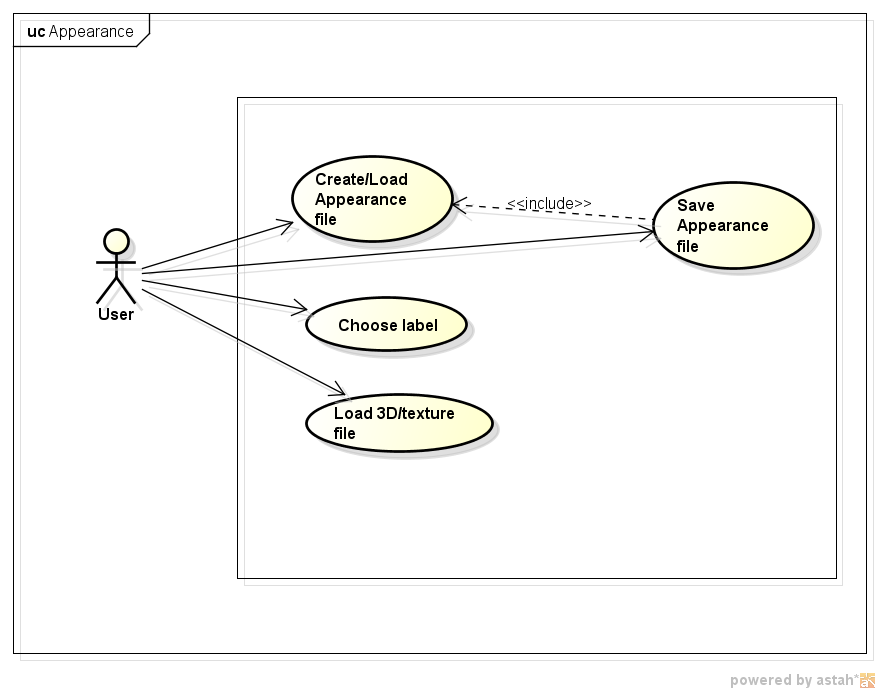
\includegraphics[width=0.8\textwidth]{image/uc-appearance.png}
  \caption{Use cases for the Appearance Editor}
  \label{fig:use-cases-appearance-editor}
\end{center}
\end{figure}


\subsection{Configuration Editor}
\writer{Albert}

The configuration editor is a component that will work as a connector between the Petri net editor (Section \ref{sec:sf-petrinet}), the Geometry editor (Section \ref{sec:sf-geometry}) and the Appearance editor (Section \ref{sec:sf-appearance}). 

\subsubsection{Functional Requirements}

\begin{enumerate}
	\item The configuration editor \textbf{shall} allow the user to input a Petri net file containing its model.
	\item The configuration editor \textbf{shall} allow the user to input a Geometry file containing its model.
	\item The configuration editor \textbf{shall} allow the user to input an Appearance file containing its model.
	\item The configuration editor \textbf{shall} allow the user to start a simulation with the referenced Petri net, Geometry and Appearance models.
	\item It \textbf{would be nice} if the configuration editor allows the user to validate the data.
	\item It \textbf{would be nice} if the configuration editor to save and load a specific configuration to a file.
\end{enumerate}
\subsection{3D Simulator}
\label{sec:sf-simulator}
The functionality of the 3D simulator can be specified using the following statements:
\begin{enumerate}
\item The simulator \textbf{shall} allow the user to play the simulation.
\item The simulator \textbf{shall} allow the user to pause the simulation.
\item The simulator \textbf{shall} allow the user to reset the simulation.
\item The simulator \textbf{shall} allow the user to add tokens on input places.
\item The simulator \textbf{shall} allow the user to exit the simulation.
\item The simulator \textbf{should} allow the user to change the orientation of the view.
\item It \textbf{would be nice} if the simulator allowed the user to take screenshots.
\item It \textbf{would be nice} if the simulator allowed the user to forward the simulation.
\item It \textbf{would be nice} if the simulator allowed the user to rewind the simulation.
\end{enumerate}
\section{Non functional requirements}
%\writer{Thibaud}


\subsection{Implementation constraints}

\subsection{Documentation}

\subsection{Quality Assurance}
\section{User Interface}
\label{sec:user-interface}
\writer{Morten}

The following section will describe how the Graphical User Interfaces (GUIs) of the Petri net editor, Geometry editor, Appearance editor, Configuration editor and the Simulation window should look like. How to execute different tasks in the editors, such as creating and editing Geometries and Petri nets, will be described in the handbook. 

The different editors will strive towards being intuitive for the targeted user, e.g. the Geometry editor should be easy to use for the non-technical user, while the Petri net editor should be intuitive for the Petri net engineer.

\subsection{Technologies}
The editors will be implemented as extensions to Eclipse, which allows us to use the different features that come with Eclipse. The functionality listed below is part of Eclipse and will be used for this software.

\begin{itemize}
\item{\textbf{Editor:} Used for the Petri net editor and the Geometry editor. Gives the user the ability to create and edit Petri nets and geometries.}
\item{\textbf{View:} Used to show properties of the object selected in the editor and the project files.}
\item{\textbf{Dialog:} A pop-up window used when the user has to specify a property of an object or to select textures or 3D files in the Appearance editor.}
\item{\textbf{Wizard:} A pop-up window with several pages that guides the user to fill out information correctly. Used to set up the configuration for the simulator.}
\end{itemize}

The use of these features will be further explained in the user handbook. 

\subsection{Graphical User Interface}
This section will describe the GUIs for the editors and the simulation tool. 

\subsubsection{Introduction to Petri net editor \& Geometry editor.}
The Petri net and Geometry editors are very much alike. They have the same composition and only the objects that can be drawn on the canvas are different. Both editors allow the use of two kinds of editing views: a \textit{tree editor} and a \textit{diagram editor}. On one hand, the diagram editor consist of a palette, a view with the project files, a view with the properties of the selected object and a canvas. On the other hand, the tree editor has the project explorer, the properties view and a view with the objects tree. Examples of Petri net and Geometry editors can be seen in figure \ref{fig:petrinet_tree} \& \ref{fig:petrinet_diagram} and figure \ref{fig:geometry_tree} \& \ref{fig:geometry_diagram} respectively. 

\begin{figure}[H]
\begin{center}
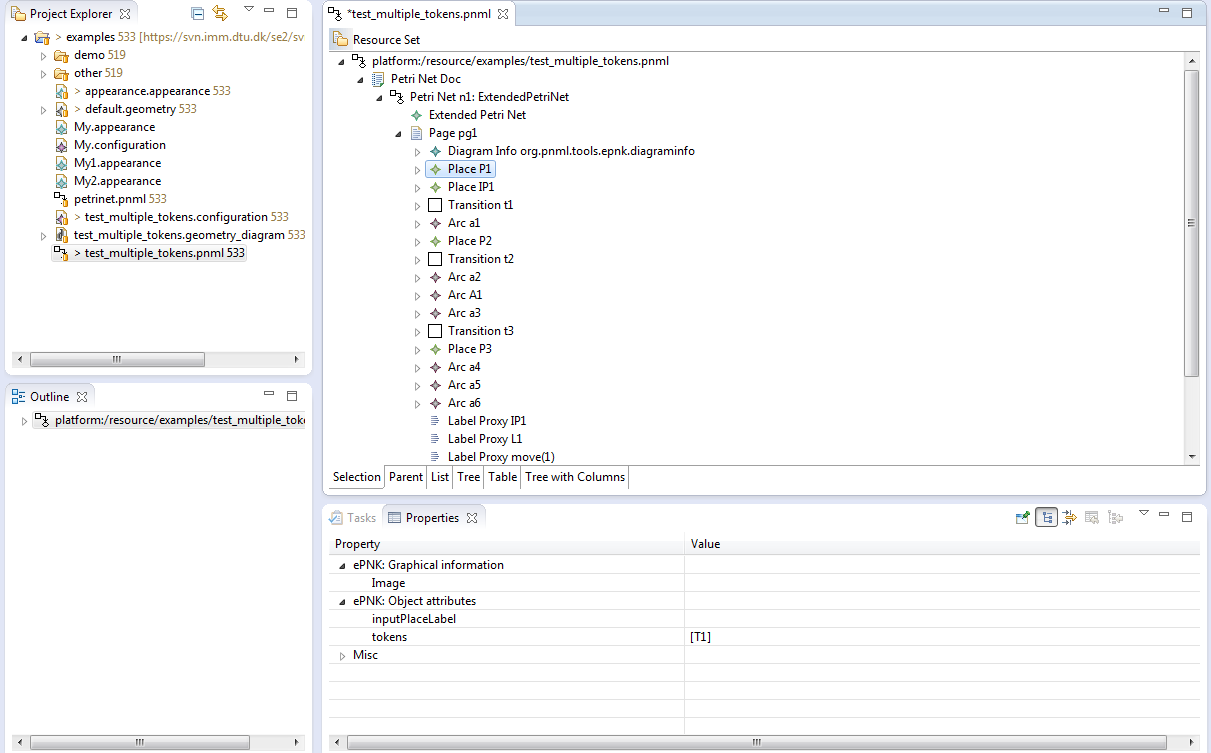
\includegraphics[scale=0.45]{image/ui/petrinet_tree.png}
\caption{The Petri net tree editor.}
\label{fig:petrinet_tree}
\end{center}
\end{figure}

\begin{figure*}[H]
\begin{center}
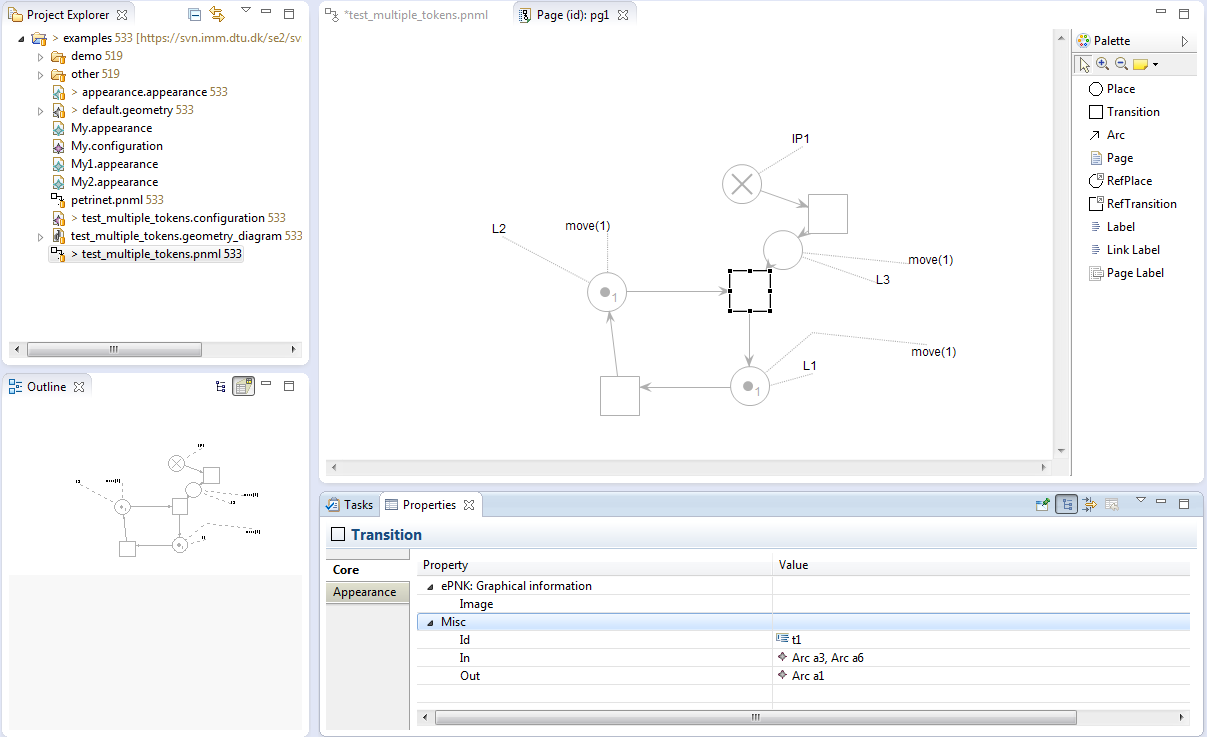
\includegraphics[scale=0.45]{image/ui/petrinet_diagram.png}
\caption{The Petri net diagram editor.}
\label{fig:petrinet_diagram}
\end{center}
\end{figure*}

\begin{figure}[H]
\begin{center}
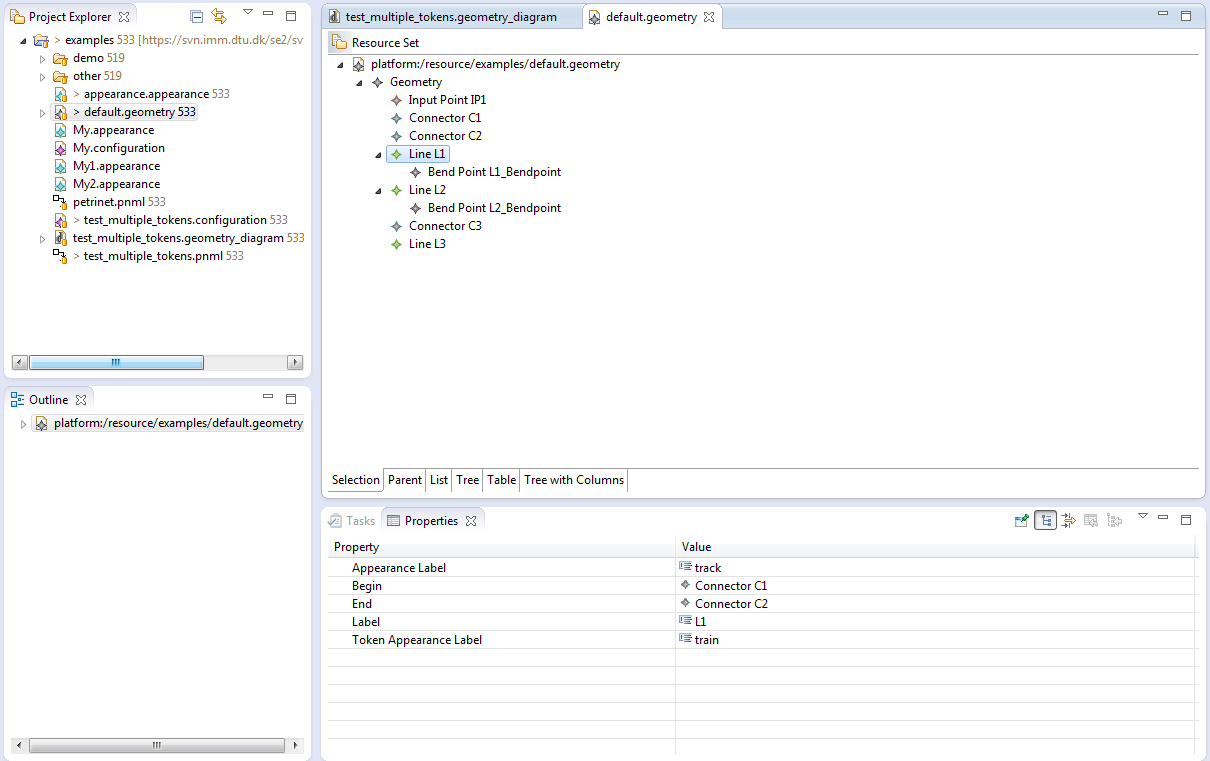
\includegraphics[scale=0.45]{image/ui/geometry_tree.png}
\caption{The geometry tree editor.}
\label{fig:geometry_tree}
\end{center}
\end{figure}

\begin{figure*}[H]
\begin{center}
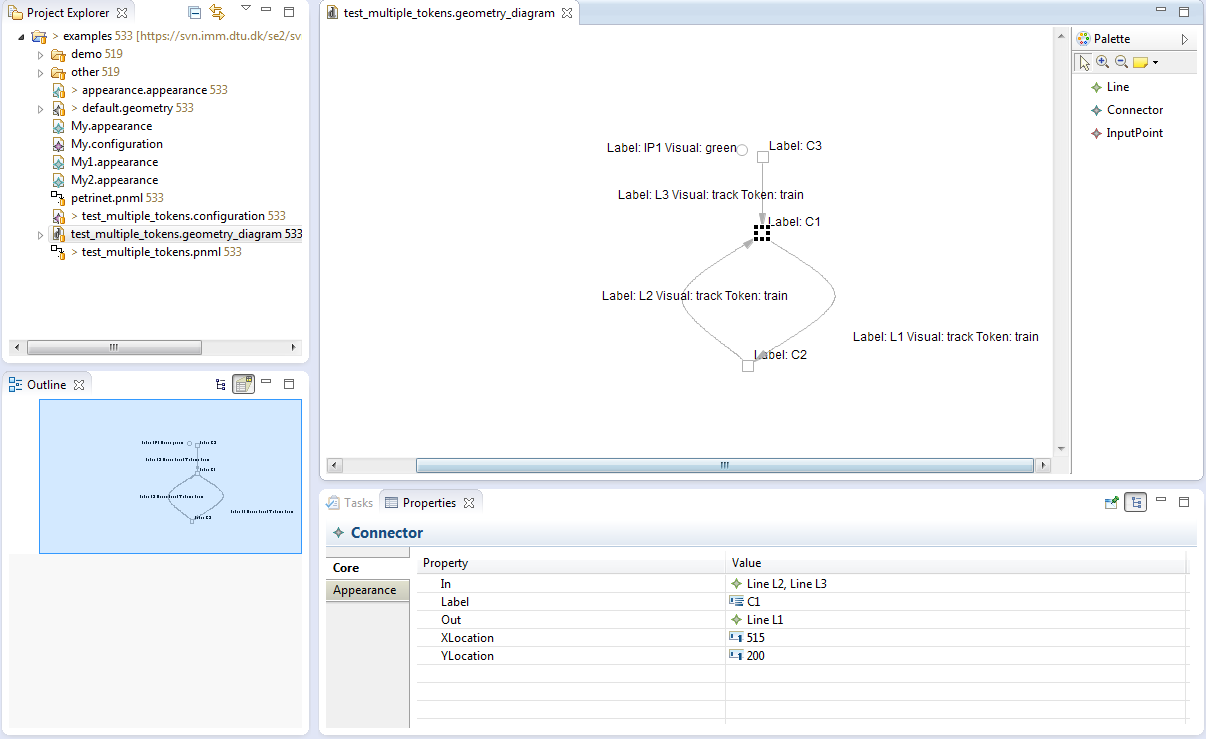
\includegraphics[scale=0.45]{image/ui/geometry_diagram.png}
\caption{The geometry diagram editor.}
\label{fig:geometry_diagram}
\end{center}
\end{figure*}

\subsubsection{Petri net editor}
\textbf{Project explorer} \\
On the left side, the user will have a view where all the files associated to the project are shown. This view will be able to identify the type of each file and, when the user opens one of the files, the editor associated to the file type will open accordingly. 

\textbf{Canvas (diagram editor)} \\
The canvas is the place where the user can create/draw the Petri net. In the diagram editor the user selects an object from the palette and left-clicks on the canvas to create the object. The user can edit the position of the different objects by dragging them around the canvas. Furthermore, the connections between the objects can be edited by dragging lines between two objects (while following the rules of the Petri net). The user will be able to see the graphical representation of the Petri net in the Petri net diagram editor. 

\textbf{Palette} \\
To create and modify the Petri net the user will be able to create objects on the canvas by selecting the desired tool in the palette on the right side. The palette in the Petri net editor has tools to create places, transitions and arcs. Each object will have a dedicated icon in order to increase the usability of the GUI.

\textbf{Tree editor} \\
In the tree editor the user can create objects by right-clicking and selecting Add object. The tree editor gives the user a quick overview of how the different objects are connected in a hierarchical manner.

\textbf{Object properties} \\
Each object has different properties that can be defined by the user. The user can modify these properties in the properties view whenever an object is selected. The Petri net objects have the following properties: \\
\textbf{Transition}
\begin{itemize}
\item{\textbf{Id:} The id of the object used in the simulator.}
\item{\textbf{In:} The incoming arcs.}
\item{\textbf{Out:} The outgoing arcs.}
\end{itemize}
\textbf{Place}%%%%%%%%%%%%
\begin{itemize}
\item{\textbf{Id:} The id of the object used in the simulator.}
\item{\textbf{In:} The incoming arcs.}
\item{\textbf{Out:} The outgoing arcs.}
\item{\textbf{Tokens:} A list of tokens placed on this place.}
\item{\textbf{Input place label:} Determines whether the place is an input place. Can either be true of false.}
\end{itemize}
\textbf{Arc}%%%%%%%%%%%%
\begin{itemize}
\item{\textbf{Id:} The id of the object used in the simulator.}
\item{\textbf{Source:} The source object.}
\item{\textbf{Target:} The target object.}
\end{itemize}

\subsubsection{Geometry editor}
\textbf{Project explorer} \\
On the left side, the user will have a view where all the files associated to the project are shown. This view will be able to identify the type of each file and, when the user opens one of the files, the editor associated to the file type will open accordingly. 

\textbf{Canvas (diagram editor)} \\
The canvas is the place where the user can create/draw the geometry. In the diagram editor the user selects an object from the palette and left-clicks on the canvas to create the object. The user can edit the position of the different objects by dragging them around the canvas. Furthermore, the connections between the objects can be edited by dragging lines between two objects. The user can create bend points on these lines to modify the slopes of the lines. The user will be able to see the graphical representation of the Petri net in the Petri net diagram editor. 

\textbf{Palette} \\
To create and modify the geometry, the user will be able to create objects on the canvas by selecting the desired tool in the palette on the right side. The palette in the geometry editor has tools to create input places, connections and lines. Each object will have a dedicated icon in order to increase the usability of the GUI.

\textbf{Object properties} \\
Each object has different properties that can be defined by the user. The user can modify these properties in the properties view whenever an object is selected. The Geometry objects have the following properties: \\
\textbf{Input point}
\begin{itemize}
\item{\textbf{Appearance label:} The appearance label is used in the appearance editor where the user specify the appearance in the 3D simulation of the specific label.}
\item{\textbf{Label:} Used in the 3D engine for recognition.}
\item{\textbf{X and Y location:} The position in the simulation.}
\end{itemize}
\textbf{Connector}
\begin{itemize}
\item{\textbf{Label:} Used in the 3D engine for recognition.}
\item{\textbf{In:} The incoming lines.}
\item{\textbf{Out:} The outgoing lines.}
\item{\textbf{X and Y location:} The position in the simulation.}
\end{itemize}
\textbf{Line}
\begin{itemize}
\item{\textbf{Appearance label:} The appearance label is used in the appearance editor where the user specify the appearance in the 3D simulation of the specific label.}
\item{\textbf{Begin:} The source connector.}
\item{\textbf{End:} The target connector.}
\item{\textbf{Label:} Used in the 3D engine for recognition.}
\item{\textbf{Token appearance label:} The appearance label of the tokens on this line. The user specifies the appearance in the appearance editor.}
\end{itemize}

\subsubsection{Appearance editor}
Figure \ref{fig:appearance_editor} is an example of the appearance editor. The user has previously specified, in the Geometry editor, the appearance labels for each object. The user creates a new Appearance object (AObject) in the editor and gives it the same label as given in the Geometry editor. The user can specify the texture and model files of the appearance in the texture and Object3D properties.

\begin{figure}[ht]
\begin{center}
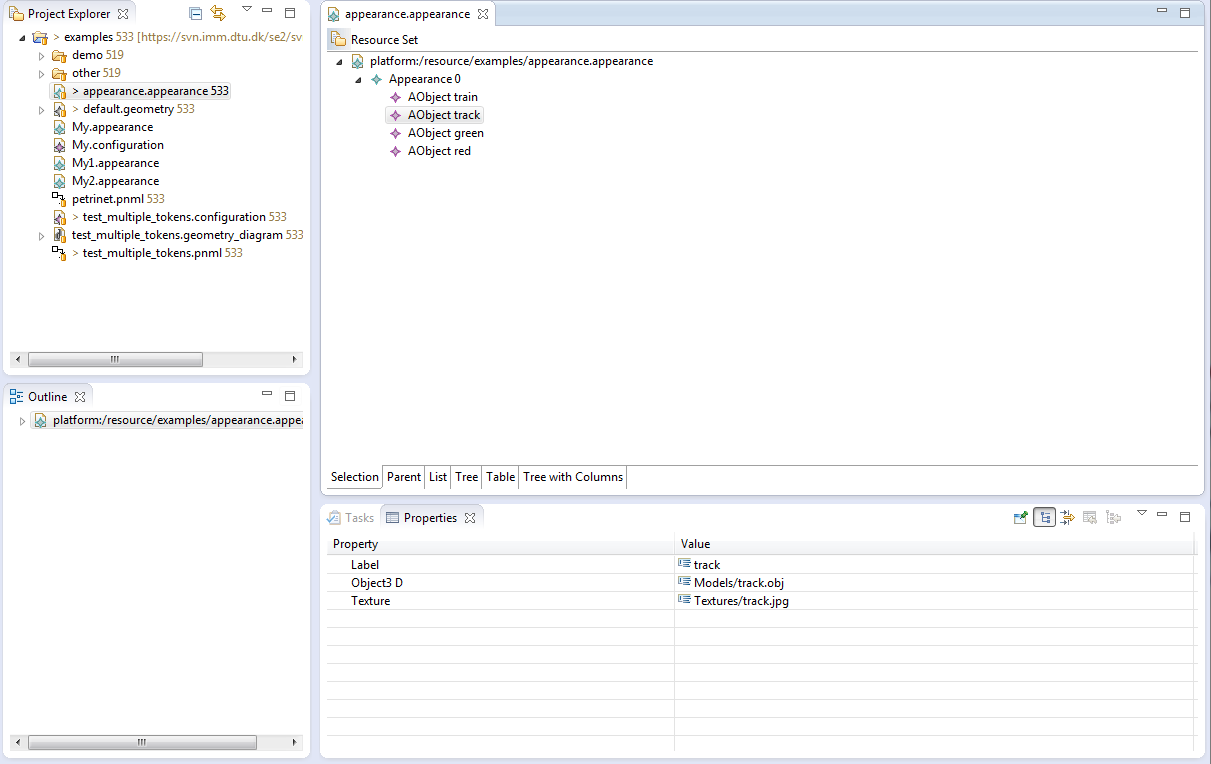
\includegraphics[scale=0.45]{image/ui/appearance.png}
\caption{The Appearance editor GUI.}
\label{fig:appearance_editor}
\end{center}
\end{figure}

\subsubsection{Configuration editor}
The configuration editor (figure \ref{fig:configuration}) helps the user to set up the 3D simulation. In the editor the user has to specify the Petri net, the geometry and the appearance files that he/she wants to use for the 3D simulation. In this way the user can, for example, have different Petri nets but still use the same visual representation for tokens and places in the simulator.

\subsubsection{Simulation tool}
When the user has successfully set up the Configuration, he will be able to run the 3D simulation. The 3D simulation opens in a new window. This window has a \textbf{play/pause} button that changes according to the state of the system; if the simulation state is play the button will be a pause symbol and the other way around. The window also has a \textbf{reset} button that allows the user to reset the simulation.
Moreover, the user will be able to interact with the simulation, therefore the user will be able to use the mouse to click on different objects. Last but not least, the user will also be able to use the mouse and keyboard to change the camera perspective. An example of the simulation tool can be seen in Figure \ref{fig:simulation_tool}.

\begin{figure}[ht]
\begin{center}
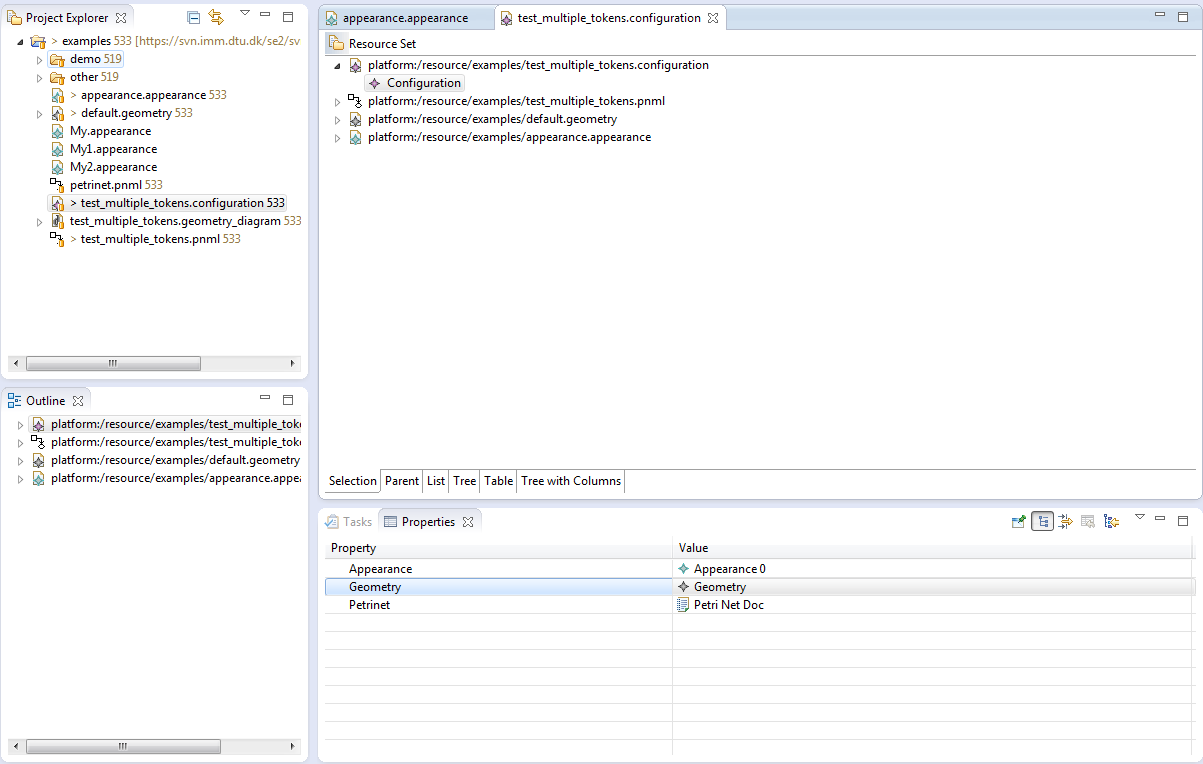
\includegraphics[scale=0.45]{image/ui/configuration.png}
\caption{The configuration editor.}
\label{fig:configuration}
\end{center}
\end{figure}

\begin{figure}[ht]
\begin{center}
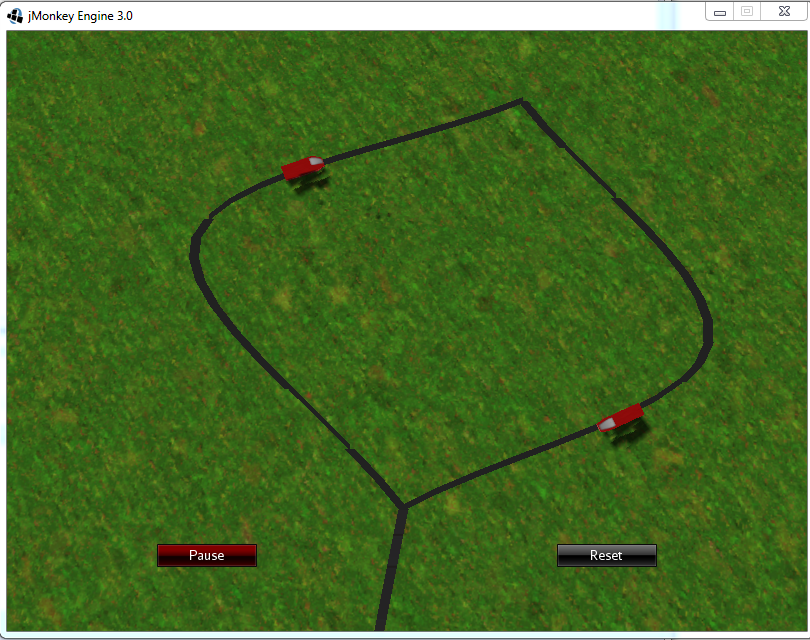
\includegraphics[scale=0.5]{image/ui/simulator.png}
\caption{An example of the Simulation tool.}
\label{fig:simulation_tool}
\end{center}
\end{figure}

\section{Architecture}
\section{Glossary}
\begin{description}

\item [3D] Three dimensional.

\item [Bendpoint] Bendpoint is a point, which functions as a control point for parametric curves allowing “bending” of said curve.

\item [Bézier-curve] Bézier-curve is a parametric curve, where shape is defined by blend of different control points.

\item [Catmull-rom] Catmull-rom splines are a family of cubic interpolating splines formulated such that tangent at each point of the spline is calculated using the previous and next point on the spline. (http://www.cs.cmu.edu/~462/projects/assn2/assn2/catmullRom.pdf)

\item [Connector]  Connector serves as either first or the last point of line.

\item [ePNK] Eclipse Petri Net Kernel.

\item [Geometry object] Geometry object can be either point or line.

\item [GUI] Graphical User Interface

\item [Input Point] Input Point is a point, where user is allowed to add tokens during the simulation.

\item [Javadoc standard] Format used by Javadoc is the industry standard for documenting Java classes.

\item [Parametric curve] Parametric curve is a mathematical curve defined by point locations.

\item [Petri net] A mathematical and graphical model for the description of distributed systems. It is a directed bipartite graph, in which nodes represent transitions and places. The directed arcs describe which places are pre- and/or post-conditions for which transitions. [source wiki]

\item [Point] Point is a coordinate location in a two dimensional plane.

\item [Token] Petri net element which moves along the Petri net places through transitions.

\item [UML] Unified Modeling Language - standardized, general-purpose modeling language in the field of software engineering. [source wiki]

\item [Use case] A list of steps defining interactions between a role (e.g. "technical user"), also known as an actor, and a system for achieving a goal. The actor can be a human or an external system.





 \end{description}

\printindex

\end{document}

